\newpage
\section{Suggested solutions: Complex Algebra}
\begin{enumerate}

\item Euler's formula:
$$e^{i\theta}=\cos\theta+i\sin\theta,$$
so for $\theta=\pi$,
$$e^{\pi i}=\cos(\pi)+i\sin(\pi)=-1,$$
as $\cos(\pi)=-1$ and $\sin(\pi)=0$, hence $e^{\pi i}+1=0$. 

\item Multiply by $i$ in the numerator and denominator to obtain:
$$\frac{1}{i}=\frac{i}{i^{2}}=-i.$$
Using Euler's formula $e^{i\theta}=\cos\theta+i\sin\theta$ we take $\theta=\frac{3\pi}{2}$, this gives a polar representation of $-i$ as:
$$-i=e^{\frac{3\pi}{2}i}.$$
\textbf{Remark}: Multiplication by $i$ rotates any vector in the complex plane 
by $\pi/2$ counterclockwise and $(1/i)(i)=1$, so $1/i$ rotates by $\pi/2$ clockwise, so our result makes sense. 

\item Use Euler's formula: $e^{i\theta}=\cos\theta+i\sin\theta$, with $\theta=\pi/2$. Then we can write $e^{\frac{\pi}{2}i}=i$ giving us:
$$i^{i}=(e^{\frac{\pi}{2}i})^{i}=e^{\frac{\pi}{2}i^{2}}=e^{-\frac{\pi}{2}}\in\mathbb{R}.$$
Thus, $i^{i}$ is a real number. 

\item Let $x$ be any real number and $n$ be an integer. Using Equation \ref{eq:complexexponentiation} we 
have $(e^{a})^{n}=\underbrace{e^{a}e^{a}\hdots e^{a}}_{n\ \text{times}}=e^{\overbrace{a+a+\hdots+a}^{n\ \text{times}}}=e^{an}$ therefore:
$$[\cos(x)+i\sin(x)]^{n}=(e^{ix})^{n}=e^{ixn}=\cos(nx)+i\sin(nx),$$
as desired. 

\item From the hint we have that $e^{i2\pi k}=1$ which can be combined with 
the fact that $(e^{a})^{n}=e^{an}$, giving that the solutions to $z^{n}=1$ are of the form:
$$w_{k}=e^{\frac{2\pi i k}{n}}, \quad k=0,\hdots,n-1.$$
A simple check to see that this is what we want is that $w_{k}$ satisfy:
$$(w_{k})^{n}=(e^{\frac{2\pi ik}{n}})^{n}=e^{2\pi ik}.$$
This gives $1$ since $e^{2\pi ik}=1$ for all $k\in\mathbb{Z}$. 
This gives $n$ unique solutions to the equation, $z^{n}=1$ as expected by the fundamental theorem of algebra.  

\item Referring to the previous problem.
\begin{itemize}
    \item[a)] Have that $w_{k}=e^{2\pi ik/5}$ for $k=0,1,2,3,4$. 
    \item[b-c)] See Listing \ref{exercise3.6}. The figure formed by the fifth roots of unity is a regular pentagon. 
\end{itemize}

\lstinputlisting[language=Python,caption={Solution for Exercise 3.6},label=exercise3.6]{ch03/code/ex3.6.py}

\begin{marginfigure}
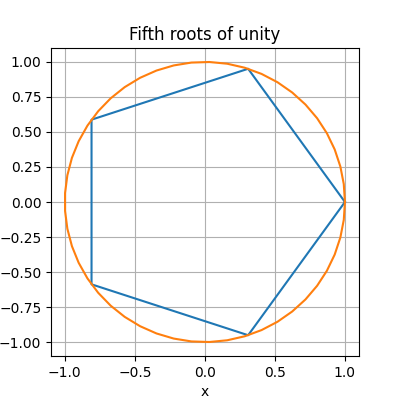
\includegraphics[width=7.5cm,height=7.0cm]{ch03/code/roots}
\end{marginfigure}

\item Have that:
\begin{align*}
    \cos(\theta)&=\frac{1}{2}(e^{i\theta}+e^{-i\theta}), \\
    \sin(\theta)&=\frac{1}{2i}(e^{i\theta}-e^{-i\theta}).
\end{align*}
Using that $1/i=-i$ from Exercise 2 we get:
$$(1-i)e^{-i\omega t}+(1+i)e^{i\omega t}=(e^{i\omega t}+e^{-i\omega t})-\frac{1}{i}(e^{i\omega t}-e^{-i\omega t}).$$
By the inverse Euler relations we may write this as:
$$(1-i)e^{-i\omega t}+(1+i)e^{i\omega t}=2\cos(\omega t)-2\sin(\omega t).$$
Next step is to write this as a pure cosine. That is, determine $A$ and $\phi$ such that:
$$A\cos(\omega t+\phi)=2\cos(\omega t)-2\sin(\omega t).$$
Using $\cos(\alpha+\beta)=\cos(\alpha)\cos(\beta)-\sin(\alpha)\sin(\beta)$ this can be rewritten as:
$$A\cos(\omega t)\cos(\phi)-A\sin(\omega t)\sin(\phi)=2\cos(\omega t)-2\sin(\omega t).$$
Therefore, $A$ and $\phi$ must satisfy:
\begin{align*}
    A\cos(\phi) &= 2, \\
    A\sin(\phi) &= 2.
\end{align*}
In other words $A=\sqrt{2^{2}+2^{2}}=\sqrt{8} = 2\sqrt{3}$ and $\tan(\phi) = 1$. 
With $\phi$ in the first quadrant, this gives $\phi=\pi/4$. Hence:
$$(1-i)e^{-i\omega t} + (1+i)e^{i\omega t} = 2\sqrt{3}\cos\left(\omega t+\frac{\pi}{4}\right).$$

\item Replace the cosine to obtain:
$$\cos(3\theta)=\frac{1}{2}(e^{3i\theta}+e^{-3i\theta})=\frac{1}{2}((e^{i\theta})^{3}+(e^{-i\theta})^{3}).$$
When expanded the first term is:
$$(\cos\theta+i\sin\theta)^{3}=\cos^{3}\theta+3i\cos^{2}\theta\sin\theta-3\cos\theta\sin^{2}\theta-i\sin^{3}\theta,$$
and the second term:
$$(\cos\theta-i\sin\theta)^{3}=\cos^{3}\theta-3i\cos^{2}\theta\sin\theta-3\cos\theta\sin^{2}\theta+i\sin^{3}\theta.$$
Adding these together then gives:
$$\cos(3\theta)=\cos^{3}\theta-3\cos\theta\sin^{2}\theta.$$

\item Let $z_{1}=e^{\alpha i}$ and $z_{2}=e^{\beta i}$ be complex numbers. Then:
$$z_{1}z_{2}=e^{\alpha i}e^{\beta i}=e^{(\alpha+\beta)i}=\cos(\alpha+\beta)+i\sin(\alpha+\beta).$$
In addition, we have that:
$$e^{\alpha i}e^{\beta i}=(\cos\alpha+i\sin\alpha)(\cos\beta+i\sin\beta)=(\cos\alpha\cos\beta-\sin\alpha\sin\beta)+i(\sin\alpha\cos\beta+\cos\alpha\sin\beta).$$
Taking the real and imaginary parts we get that:
\begin{align*}
    \cos(\alpha+\beta) &=\cos\alpha\cos\beta-\sin\alpha\sin\beta, \\
    \sin(\alpha+\beta) &=\sin\alpha\cos\beta+\cos\alpha\sin\beta.
\end{align*}

\item Consider the complex exponential of the form $e^{i\theta}$, then by this new definition we have:
$$e^{i\theta}=\sum_{k=0}^{\infty}\frac{(i\theta)^{k}}{k!}.$$
Using this definition we have:
$$e^{i\theta}=\sum_{k=0}^{\infty}\frac{(i\theta)^{k}}{k!}=1 + i\theta + \frac{(i\theta)^{2}}{2!} + \frac{(i\theta)^{3}}{3!} + \frac{(i\theta)^{4}}{4!} + \hdots.$$
Using that $i^{2}=-1$ we get:
$$e^{i\theta}=1+i\theta-\frac{\theta^{2}}{2!}-i\frac{\theta^{3}}{3!}+\frac{\theta^{4}}{4!}+\hdots$$
Grouping terms with and without $i$ this can be written as:
$$e^{i\theta}=(1-\frac{\theta^{2}}{2!}+\frac{\theta^{4}}{4!}+\hdots)+i(\theta-\frac{\theta^{3}}{3!}+\frac{\theta^{5}}{5!}-\hdots).$$
The first terms correspond to the Taylor series for $\cos \theta$ and the other $\sin \theta$, hence we get Euler's formula:
$$e^{i\theta}=\cos\theta+i\sin\theta.$$

\end{enumerate}
